%----------------------------------------------------------
\def\notedate{2023.02.28}
\def\currentauthor{Василян А.Р. (РК6-83Б)}
%----------------------------------------------------------
\notestatement{rndhpcgui}{Генерация страницы на основе данных в формате aINI}


<<<<<<< .mine
Во время разработки программы преобразования данных из aINI в HTML использовался модуль синтаксического анализа для языка Python - Pyparsing.

=======
Была разработана программа для преобразования данных формата \textsf{aINI} в \textsf{HTML}-код.
Во время разработки программы преобразования данных из \textsf{aINI} в \textsf{HTML} использовался модуль синтаксического анализа для языка \textsf{Python} - \textsf{Pyparsing}. 
>>>>>>> .theirs

<<<<<<< .mine
Программа построчно читает данные из входного файла и распознает строку в соответствии с шаблонами в парсере (листинг~\ref{rndhpcgui.2023.02.28.parser}). Интерпретация строк происходит с помощью функции \textsf{parsing} (листинг~\ref{rndhpcgui.2023.02.28.parsing}), которая принимает строку, разбирает её и возвращает список ``слов'' и ``текстов'' (построенных на основе комментариев).% и номера распознанного элемента для дальнещей генерации.
=======

>>>>>>> .theirs

<<<<<<< .mine
\begin{lstlisting}[frame=single, label={rndhpcgui.2023.02.28.parser}, caption={Парсер}, language={Python}]






=======
На листинге~\ref{rndhpcgui.2023.02.28.parser} предсталвлены парсеры для отдельных символов, текстов, а потом из отдельных частей получается парсер для строк, соответствующих определённым элементам интерфейса.


Программа построчно читает данные из входного файла и распознает строку в соответствии с шаблонами в парсере (листинг~\ref{rndhpcgui.2023.02.28.parser}). Расспознавание строк происходит в функции \textsf{parsing} (листинг~\ref{rndhpcgui.2023.02.28.parsing}) с помощью \textsf{parseString.asList()}, которая в зависимости от выбранного парсера разделяет строку на список. Функция возвращает этот список и номер распознанного элемента для дальнещей генерации.


\begin{lstlisting}[frame=single, label={rndhpcgui.2023.02.28.parser}, caption={Парсер}, language={Python}] 
>>>>>>> .theirs
	rus_alphas = 'ёйцукенгшщзхъфывапролджэячсмитьбюЁЙЦУКЕНГШЩЗХЪФЫВАПРОЛДЖЭЯЧСМИТЬБЮ'

	bool_var = Word('0' + '1')
	word_num = Word(nums + alphas)
	rus_eng_word_num = Word(alphas + rus_alphas + ' ' + nums)
	link = Word(alphanums + '-' + '+' + '=' + '/' + '.' + '_' + '#' + ':' + '&' + '?' + '%')
	text = Word(printables + rus_alphas + ' ')
	
	parse_section = '[' + word_num + ']' + '//' + rus_eng_word_num
	parse_text_box = word_num + '=' + word_num + '//' + rus_eng_word_num
	parse_box = word_num + '=' + '[' + bool_var + ']' + '{0|1}' + '//' + rus_eng_word_num
	parse_file_selection = word_num + '=' + '[file]' + '//' + rus_eng_word_num
	parse_link = '[' + link + ']' + '//' + rus_eng_word_num
	parse_text = '//' + OneOrMore(text)
\end{lstlisting}

<<<<<<< .mine
\begin{lstlisting}[frame=single, label={rndhpcgui.2023.02.28.parsing}, caption={Функция parsing}, language={Python}]

=======

\begin{lstlisting}[frame=single, label={rndhpcgui.2023.02.28.parsing}, caption={Функция parsing}, language={Python}] 
>>>>>>> .theirs
	def parsing(s):
    try:
        test = parse_section.parseString(s).asList()
        patern_id = 1
        print(1)
    except ParseException:
        try:
            test = parse_text_box.parseString(s).asList()
            patern_id = 2
            print(2)
        except ParseException:
            try:
                test = parse_box.parseString(s).asList()
                patern_id = 3
                print(3)
            except ParseException:
                try:
                    test = parse_file_selection.parseString(s).asList()
                    patern_id = 4
                    print(4)
                except ParseException:
                    try:
                        test = parse_link.parseString(s).asList()
                        patern_id = 5
                        print(5)
                    except ParseException:
                        try:
                            test = parse_text.parseString(s).asList()
                            patern_id = 6
                            print(6)
                        except ParseException:
                            print('The string is not parsed')
                            quit()
    return [patern_id, test]
\end{lstlisting}


На основе элементов списка в выходной файл записывается HTML-код с помощью соответствующих функций для каждого из предусмотренных элементов интерфейса (листинг~\ref{rndhpcgui.2023.02.28.generation}). Каждая из функций получает на фход список, из которого берутся ключевые слова для написания кода.


\begin{lstlisting}[frame=single, label={rndhpcgui.2023.02.28.generation}, caption={Функции записи HTML-кода элементов интерфейса}, language={Python}]
	def section_to_html(f, parsed_line):
    if len(parsed_line) != 5:
        section = parsed_line[1]
    else:
        section = parsed_line[4]
    f.write('<h1>'+section+'</h1>\n')

def textbox_to_html(f, parsed_line):
    if len(parsed_line) != 5:
        textbox = parsed_line[0]
    else:
        textbox = parsed_line[4]
    f.write('<p><b>'+textbox+'</b><br>\n<input type="text" value="'+parsed_line[2]+'"></p>\n')

def box_to_html(f, parsed_line):
    if len(parsed_line) != 8:
        box = parsed_line[0]
    else:
        box = parsed_line[7]
    if parsed_line[3] == '1':
        f.write('<p><<input type="checkbox" name="'+box+'" checked>'+box+'</p>\n')
    else:
        f.write('<p><<input type="checkbox" name="'+box+'">'+box+'</p>\n')

def file_selection_to_html(f, parsed_line):
    if len(parsed_line) != 5:
        file_selection = parsed_line[0]
    else:
        file_selection = parsed_line[4]
    f.write('<p><b>'+file_selection+'</b><br>\n<input type="file" name="file"></p>\n')

def link_to_html(f, parsed_line):
    if len(parsed_line) != 5:
        link_title = parsed_line[1]
    else:
        link_title = parsed_line[4]
    f.write('<p><a href="'+parsed_line[1]+'">'+link_title+'</a></p>\n')

def text_to_html(f, parsed_line):
    f.write('<p class="text">'+parsed_line[1]+'</p>\n')
\end{lstlisting}


Пример входных данных представлен на листинге~\ref{rndhpcgui.2023.02.28.aINI}. На выходе при таких данных получается HTML-код на листинге~\ref{rndhpcgui.2023.02.28.HTML}

<<<<<<< .mine
\begin{lstlisting}[frame=single, label={rndhpcgui.2023.02.28.aINI}, caption={Пример входных данных}, language={aINIExample}]

=======

\begin{lstlisting}[frame=single, label={rndhpcgui.2023.02.28.aINI}, caption={Пример входных данных}] 
>>>>>>> .theirs
	[sec1]//Пункт 1
	X=VX//Параметр X
	Y=25//Параметр Y
	box=[1] {0|1}//Флажок 1
	box=[1] {0|1}//Флажок 2
	[sec1]//Пункт 2
	box=[0] {0|1}//Флажок 3
	ParametersFile=[file]//Выберите имя файла
	[https://www.google.ru]//Ссылка на Google
	//Московский государственный технический университет им. Н. Э. Баумана - российский национальный исследовательский университет, научный центр, особо ценный объект культурного наследия народов России.
\end{lstlisting}

<<<<<<< .mine































=======

\begin{lstlisting}[frame=single, label={rndhpcgui.2023.02.28.HTML}, caption={Пример выходных данных}, language={HTML}] 
	<!DOCTYPE HTML>
	<html>
	<head>
	<meta charset="utf-8">
	<title>title</title>
	<style>
	p.text {text-indent: 20px;}
	</style>
	</head>
	<body>
	<form enctype="multipart/form-data" method="post">
	<h1>Пункт 1</h1>
	<p><b>Параметр X</b><br>
	<input type="text" value="VX"></p>
	<p><b>Параметр Y</b><br>
	<input type="text" value="25"></p>
	<p><<input type="checkbox" name="Флажок 1" checked>Флажок 1</p>
	<p><<input type="checkbox" name="Флажок 2" checked>Флажок 2</p>
	<h1>Пункт 2</h1>
	<p><<input type="checkbox" name="Флажок 3">Флажок 3</p>
	<p><b>Выберите имя файла</b><br>
	<input type="file" name="file"></p>
	<p><a href="https://www.google.ru">Ссылка на Google</a></p>
	<p class="text">Московский государственный технический университет им. Н. Э. Баумана - российский национальный исследовательский университет, научный центр, особо ценный объект культурного наследия народов России.</p>
	</form>
	</body>
	</html>
\end{lstlisting}

>>>>>>> .theirs

Итоговая страница на рисунке~\ref{rndhpcgui.2023.02.28.picture1}.


\begin{figure}[!ht]
  \centering
  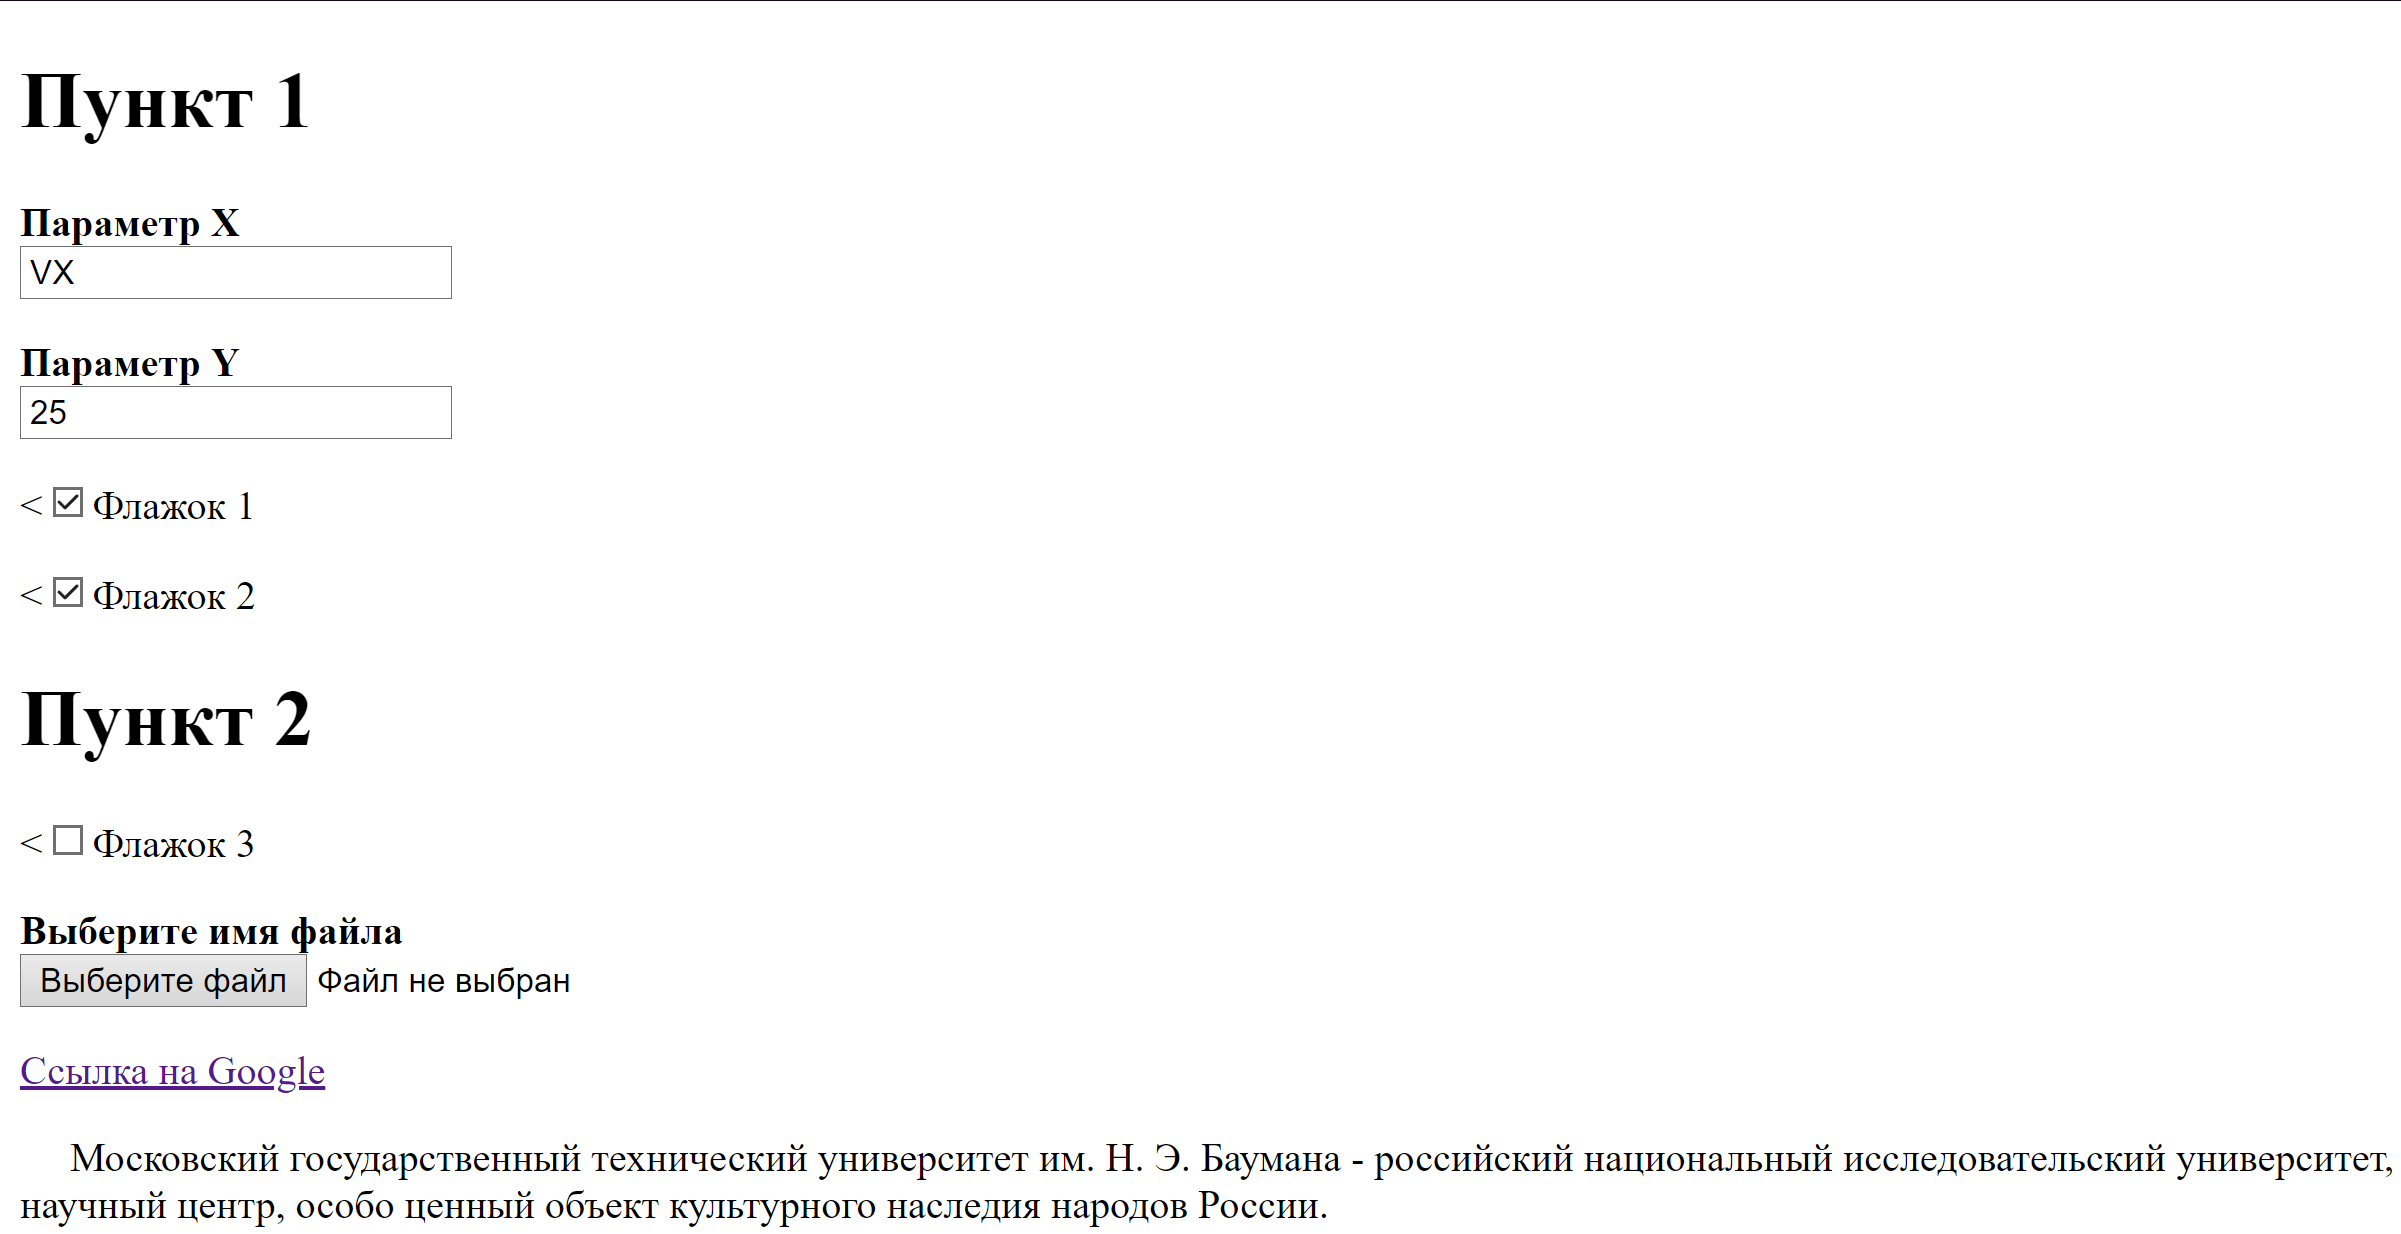
\includegraphics[scale=0.4]{ResearchNotes/rndhpc_dev_gui_2023_02_28/rndhpcgui.2023.02.28.picture1.png}
  \caption{Пример}
  \label{rndhpcgui.2023.02.28.picture1}
\end{figure}

<<<<<<< .mine
Полный код программы~\ref{rndhpcgui.2023.02.28.aINI_to_HTML}.
\begin{lstlisting}[frame=single, label={rndhpcgui.2023.02.28.aINI_to_HTML}, caption={Пример выходных данных}, language={Python}]
    from pyparsing import *
    rus_alphas = 'ёйцукенгшщзхъфывапролджэячсмитьбюЁЙЦУКЕНГШЩЗХЪФЫВАПРОЛДЖЭЯЧСМИТЬБЮ'

    bool_var = Word('0' + '1')
    word_num = Word(nums + alphas)
    rus_eng_word_num = Word(alphas + rus_alphas + ' ' + nums)
    link = Word(alphanums + '-' + '+' + '=' + '/' + '.' + '_' + '#' + ':' + '&' + '?' + '%')
    text = Word(printables + rus_alphas + ' ')

    parse_section = '[' + word_num + ']' + '//' + rus_eng_word_num
    parse_text_box = word_num + '=' + word_num + '//' + rus_eng_word_num
    parse_box = word_num + '=' + '[' + bool_var + ']' + '{0|1}' + '//' + rus_eng_word_num
    parse_file_selection = word_num + '=' + '[file]' + '//' + rus_eng_word_num
    parse_link = '[' + link + ']' + '//' + rus_eng_word_num
    parse_text = '//' + OneOrMore(text)

    def parsing(s):
        try:
            test = parse_section.parseString(s).asList()
            patern_id = 1
            print(1)
        except ParseException:
            try:
                test = parse_text_box.parseString(s).asList()
                patern_id = 2
                print(2)
            except ParseException:
                try:
                    test = parse_box.parseString(s).asList()
                    patern_id = 3
                    print(3)
                except ParseException:
                    try:
                        test = parse_file_selection.parseString(s).asList()
                        patern_id = 4
                        print(4)
                    except ParseException:
                        try:
                            test = parse_link.parseString(s).asList()
                            patern_id = 5
                            print(5)
                        except ParseException:
                            try:
                                test = parse_text.parseString(s).asList()
                                patern_id = 6
                                print(6)
                            except ParseException:
                                print('The string is not parsed')
                                quit()
        return [patern_id, test]

    def html_start():
        page_title = input('Введите название страницы\n')
        f = open(page_title + '.html', 'w', encoding='utf-8')
        f.write('<!DOCTYPE HTML>\n<html>\n<head>\n<meta charset="utf-8">\n<title>'+page_title+'</title>\n<style>\np.text {text-indent: 20px;}\n</style>\n</head>\n<body>\n<form enctype="multipart/form-data" method="post">\n')
        return f

    def section_to_html(f, parsed_line):
        if len(parsed_line) != 5:
            section = parsed_line[1]
        else:
            section = parsed_line[4]
        f.write('<h1>'+section+'</h1>\n')

    def textbox_to_html(f, parsed_line):
        if len(parsed_line) != 5:
            textbox = parsed_line[0]
        else:
            textbox = parsed_line[4]
        f.write('<p><b>'+textbox+'</b><br>\n<input type="text" value="'+parsed_line[2]+'"></p>\n')

    def box_to_html(f, parsed_line):
        if len(parsed_line) != 8:
            box = parsed_line[0]
        else:
            box = parsed_line[7]
        if parsed_line[3] == '1':
            f.write('<p><<input type="checkbox" name="'+box+'" checked>'+box+'</p>\n')
        else:
            f.write('<p><<input type="checkbox" name="'+box+'">'+box+'</p>\n')

    def file_selection_to_html(f, parsed_line):
        if len(parsed_line) != 5:
            file_selection = parsed_line[0]
        else:
            file_selection = parsed_line[4]
        f.write('<p><b>'+file_selection+'</b><br>\n<input type="file" name="file"></p>\n')

    def link_to_html(f, parsed_line):
        if len(parsed_line) != 5:
            link_title = parsed_line[1]
        else:
            link_title = parsed_line[4]
        f.write('<p><a href="'+parsed_line[1]+'">'+link_title+'</a></p>\n')

    def text_to_html(f, parsed_line):
        f.write('<p class="text">'+parsed_line[1]+'</p>\n')

    def html_finish(f):
        f.write('</form>\n</body>\n</html>')
        f.close()

    def main():
        file_name = input('Введите название читаемого файла\n')
        input_f = open(file_name, encoding='utf-8')
        f = html_start()
        for line in input_f:
            print(line)
            id_and_line = parsing(line)
            patern_id = id_and_line[0]
            parsed_line = id_and_line[1]
            print(parsed_line)
            if patern_id <= 3:
                if patern_id == 1:
                    section_to_html(f, parsed_line)
                else:
                    if patern_id == 2:
                        textbox_to_html(f, parsed_line)
                    else:
                        if patern_id == 3:
                            box_to_html(f, parsed_line)
            else:
                if patern_id == 4:
                    file_selection_to_html(f, parsed_line)
                else:
                    if patern_id == 5:
                        link_to_html(f, parsed_line)
                    else:
                        if patern_id == 6:
                            text_to_html(f, parsed_line)
        html_finish(f)

    if __name__ == '__main__':
        main()
\end{lstlisting}
=======









































































































































>>>>>>> .theirs
%----------------------------------------------------------
% Атрибуты задачи
\noteattributes{}
%----------------------------------------------------------
